%!TEX root = ../thesis.tex
\chapter{Introduction}
\label{chapter_introduction}

When attempting to accomplish unfamiliar, complicated tasks, people often look for tutorials to follow instructions. From performing daily tasks such as cooking and operating a machine, using software applications, to physical activities like sports and dance performance, each domain involves specific ``how-to'' knowledge with a certain degree of complexity~\cite{ryle1945knowhow}.
%
Instructions, which describe how a specific goal can be accomplished, are a tool for people to self-learn a task~\cite{Smith03iimanufacturer}. Studies have shown that visual instructions are cognitively favorable by people as they are easier to comprehend and remember than text information~\cite{Harrison:1995uh,mayer1996less,Heiser:2004:IVC:989863.989917}. In history, pictorial instructions have been created from the Middle Age to explain dancing or weapon operations~\cite{mijksenaar1999open}. It was found that the first use of letters in technical drawing for text referral was by Italian polymath Leonardo da Vinci. In 1737, French engineer de B{\'e}lidor~\cite{de1737architecture}'s diagrams were the first to apply arrows to indicate direction of movements (see Figure~\ref{fig:intro_arrows}).
%
From 1760, when the Industrial Revolution introduced mass production, instructions have been seen widely for various products and uses.

\begin{figure*}[h!]
  \centering
  \begin{minipage}{\textwidth}
  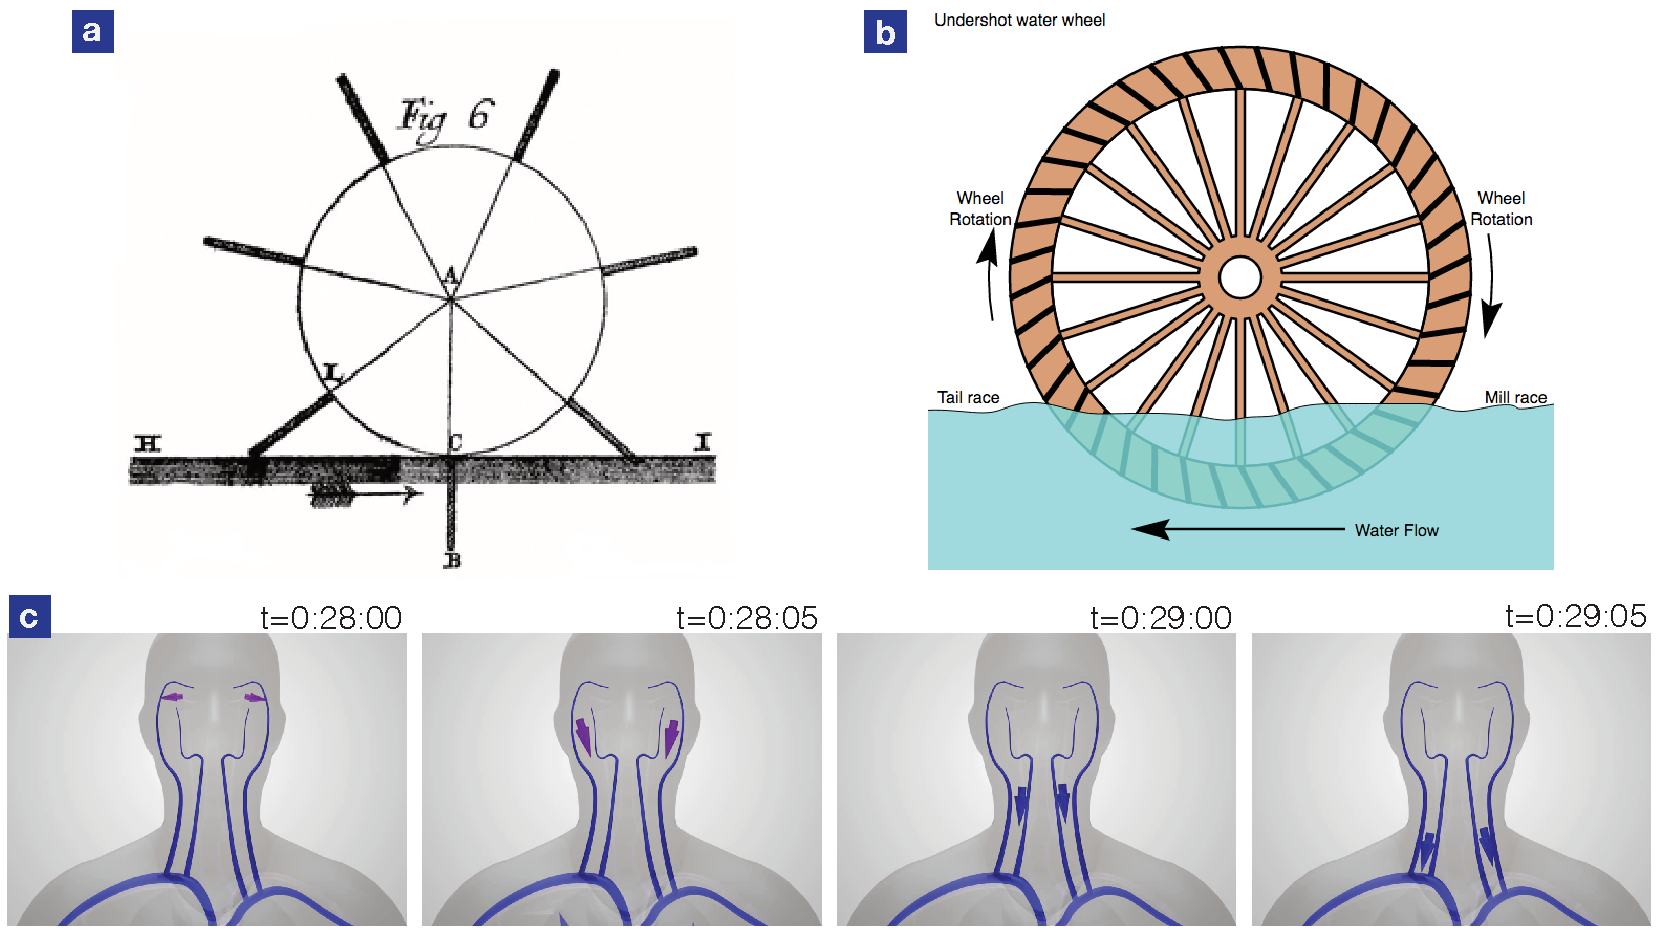
\includegraphics[width=\textwidth]{\intro/fig/arrows/arrows}
  \caption[Uses of motions arrows in visual instructions.]{Uses of motions arrows in visual instructions:
  %
  a) Year 1737: The first use of a motion arrow in an illustration explains the impact of water flow of a water wheel~\cite{de1737architecture},
  % http://www.buw-output-archiv.uni-wuppertal.de/ausgabe1/steinle/index-en.html
  %
  b) Year 2002: Similarly, arrows are used to explain the water flow and rotation of an undershot water wheel\footnote[1]{Original artwork by Daniel M. Short, ``Schematic diagram of an undershot water wheel'', licensed under CC BY-SA 2.5},
  % https://en.wikipedia.org/wiki/File:Undershot_water_wheel_schematic.svg
  %
  c) Year 2014: An animation visualizes the blood flow using motion arrows\footnote[2]{Video by Bioscience Credentials, ``Blood Flow in the Human Body'', \url{https://youtu.be/GwX41xm9esY}, licensed under CC BY 3.0}.
  }
  \label{fig:intro_arrows}
  \end{minipage}
\end{figure*}

Since the late 1990s, the advance in computer technologies has introduced more versatile instructional design. Instructions can now be created via software tools rather than hand drawing; they can include multimedia such as images and videos in several forms; they can be accessed through the Internet, as well as in hard copy.
%  the general purpose computers and the Internet
%
This advancement also enables consumers or end-users to document and share their domain knowledge~\cite{Lafreniere:2012tl}. As of today, popular tutorial sharing sites like Instructables has over 220,000 articles~\cite{InstructablesProjects}, wikiHow provides over 192,000 articles~\cite{wikiHowStatistics}, Food.com serves over 500,000 user-generated recipes with 125,000 photos~\cite{FoodComAbout}, and YouTube hosts over 285 million How-To videos\footnote{YouTube, \url{https://www.youtube.com/}, accessed June 2016}.
%
The variety of topics, content, and presentation styles provides learners more options to understand domain knowledge.
%
However, navigating a tutorial using existing tools remains inefficient for following step-by-step instructions. It can be challenging to observe details from text and images or find specific piece of information in a video through a timeline with conventional video players.
%
On the other hand, producing high-quality instructions that are easy to follow requires authoring expertise and a significant time investment. It involves several stages to design, record, and edit multimedia materials of a task using a variety of creation tools~\cite{Torrey:2007he,Tseng:2014:PVP:2598510.2598540,Muller:2009tw}.\\

The goal of this dissertation is to investigate interactive instructional design and develop computational tools that support the authoring process.
%
To contribute to computational methods of authoring user-generated instructions, two research questions that this work focuses on are:

\begin{itemize}
  \item How can authoring tools support domain experts in efficiently creating effective, high-quality instructions based on video-recorded demonstrations?
  \item How can new tutorial formats help authors better express their intent and help learners understand and follow the author's instructions?
\end{itemize}

This dissertation presents video-based computational approaches that enhance tutorial creation and consumption from author demonstrations.
We encode the current practices from professional authors into automatic algorithms and interactive techniques.
%
We develop authoring tools that follow a general workflow (see Figure~\ref{fig:general_pipeline}): An author first performs a demonstration of a task. Our systems capture videos and high-level information of the demonstration. Automatic analysis on the captured materials is performed during or after the performance. Based on the analysis, the systems integrate videos, author annotations, and automatic editing decisions to produce effective instructions. Authors can review the generated results, edit, or iteratively re-perform a task.
%
Using this workflow, our work dramatically increases the quality of amateur-produced video instructions, which in turn improves learning for viewers who interactively navigate the content.

We will introduce five interactive systems that we develop to address these challenges. These tools cover both software applications (e.g., image manipulation tasks or browser navigation) and physical activities (e.g., Do-It-Yourself projects or dance movements) for recording, editing, and replaying instructional content.

\begin{figure}[t!]
  \centering
  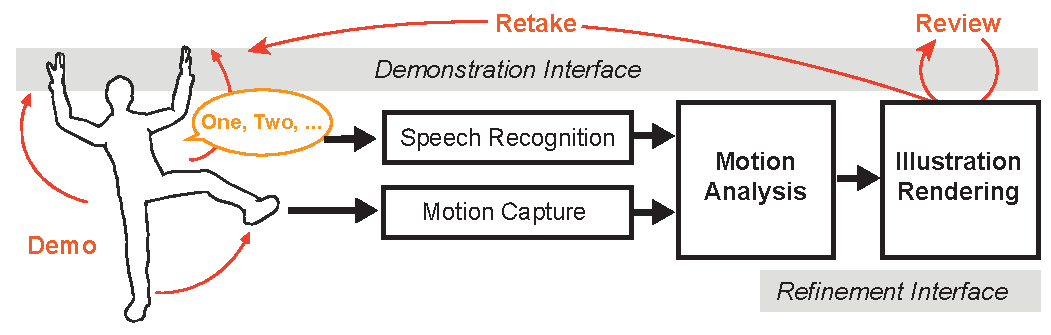
\includegraphics[width=0.8\columnwidth]{\intro/fig/pipeline}
  \caption{Our video-based approaches capture an author's demonstration, analyze the captured materials, and automatically make editing decisions to produce effective instructions. Authors can review their recordings, modify the generated results, or re-perform a demonstration.}
  \label{fig:general_pipeline}
\end{figure}

% ---------------------------------------------------------------

\section{Challenges of Creating and Consuming Instructions}

Visual instructions are the dominant form of instructional design~\cite{mijksenaar1999open}. Cognitive load theory of multimedia learning suggests that learners process information using distinct channels, one for visual and the other for verbal formats~\cite{sweller1998cognitive,sweller1988cognitive,paas2003cognitive}. It was found that learners performed better when received a pictorial summary of a scientific system than those who received the full text alone or the full text with the summary~\cite{mayer1996less}.

Among all the multimedia support, videos are a common form to present instructions. We suspect that the great popularity of videos is due to the following reasons:
%
First, consumer devices and software have become affordable for authors to quickly record activities and later share via online platforms at minimum cost.
%
% ** describe the difficulties of making knowledge "explicit", esp. for actions and motions
Second, videos can be an efficient medium to document activities. Transferring know-how concisely and effectively to the audience is challenging. It especially requires efforts when a task involves \emph{tacit knowledge}, which is a kind of knowledge that is difficult to articulate in a written or verbal form~\cite{polanyi1958personal, Klemmer:2006:BMF:1142405.1142429}. Examples of tacit knowledge include dancing, riding a bike, or driving nails with a hammer. Dancers can perform movements fluently with music. If they are asked to focus on the composite pieces, such as the arm and foot actions or rhythm, they might get confused and fail to express the entire movement~\cite{polanyi1958personal}. Very often, recording a video eases the difficulties of describing the entire activities in an explicit form.
%
This leads to another motivation that videos also provide an effective channel to convey ideas with adequate amounts of details. Learners can visually observe the exact actions in a video as if an expert were coaching in person~\cite{Kuznetsov:2010:REA:1868914.1868950}.

However, while videos are easy to produce, they can include a lot of unnecessary footage. Inevitable content such as pauses, mistakes, and long repetitive actions makes it difficult for learners to focus on the most important steps and actions. A lot of authoring effort commonly goes into extracting footage, applying visual effects, and adding subtitles and annotations.
%
In addition, even with a well-edited video, navigating using a conventional video player remains inefficient. Learners with various needs could have a hard time skimming to an interesting moment or perceiving high-level overviews. Alternatively, a pictorial summary or static step-by-step tutorials presented with text and images can effectively guide knowledgeable learners through familiar tasks.

% The goal of this dissertation to develop video-based recording, editing, and playback tools are optimized for creating and consuming instructional demonstrations. I combine the advantage of ubiquitous video recording with the benefits of video and structured tutorial formats. I aim to dramatically increase the quality of amateur-produced video instructions, which in turn improves learning for viewers who interactively navigate the content.

% ----- MixT ----- %

\begin{figure*}[b!]
  \centering
  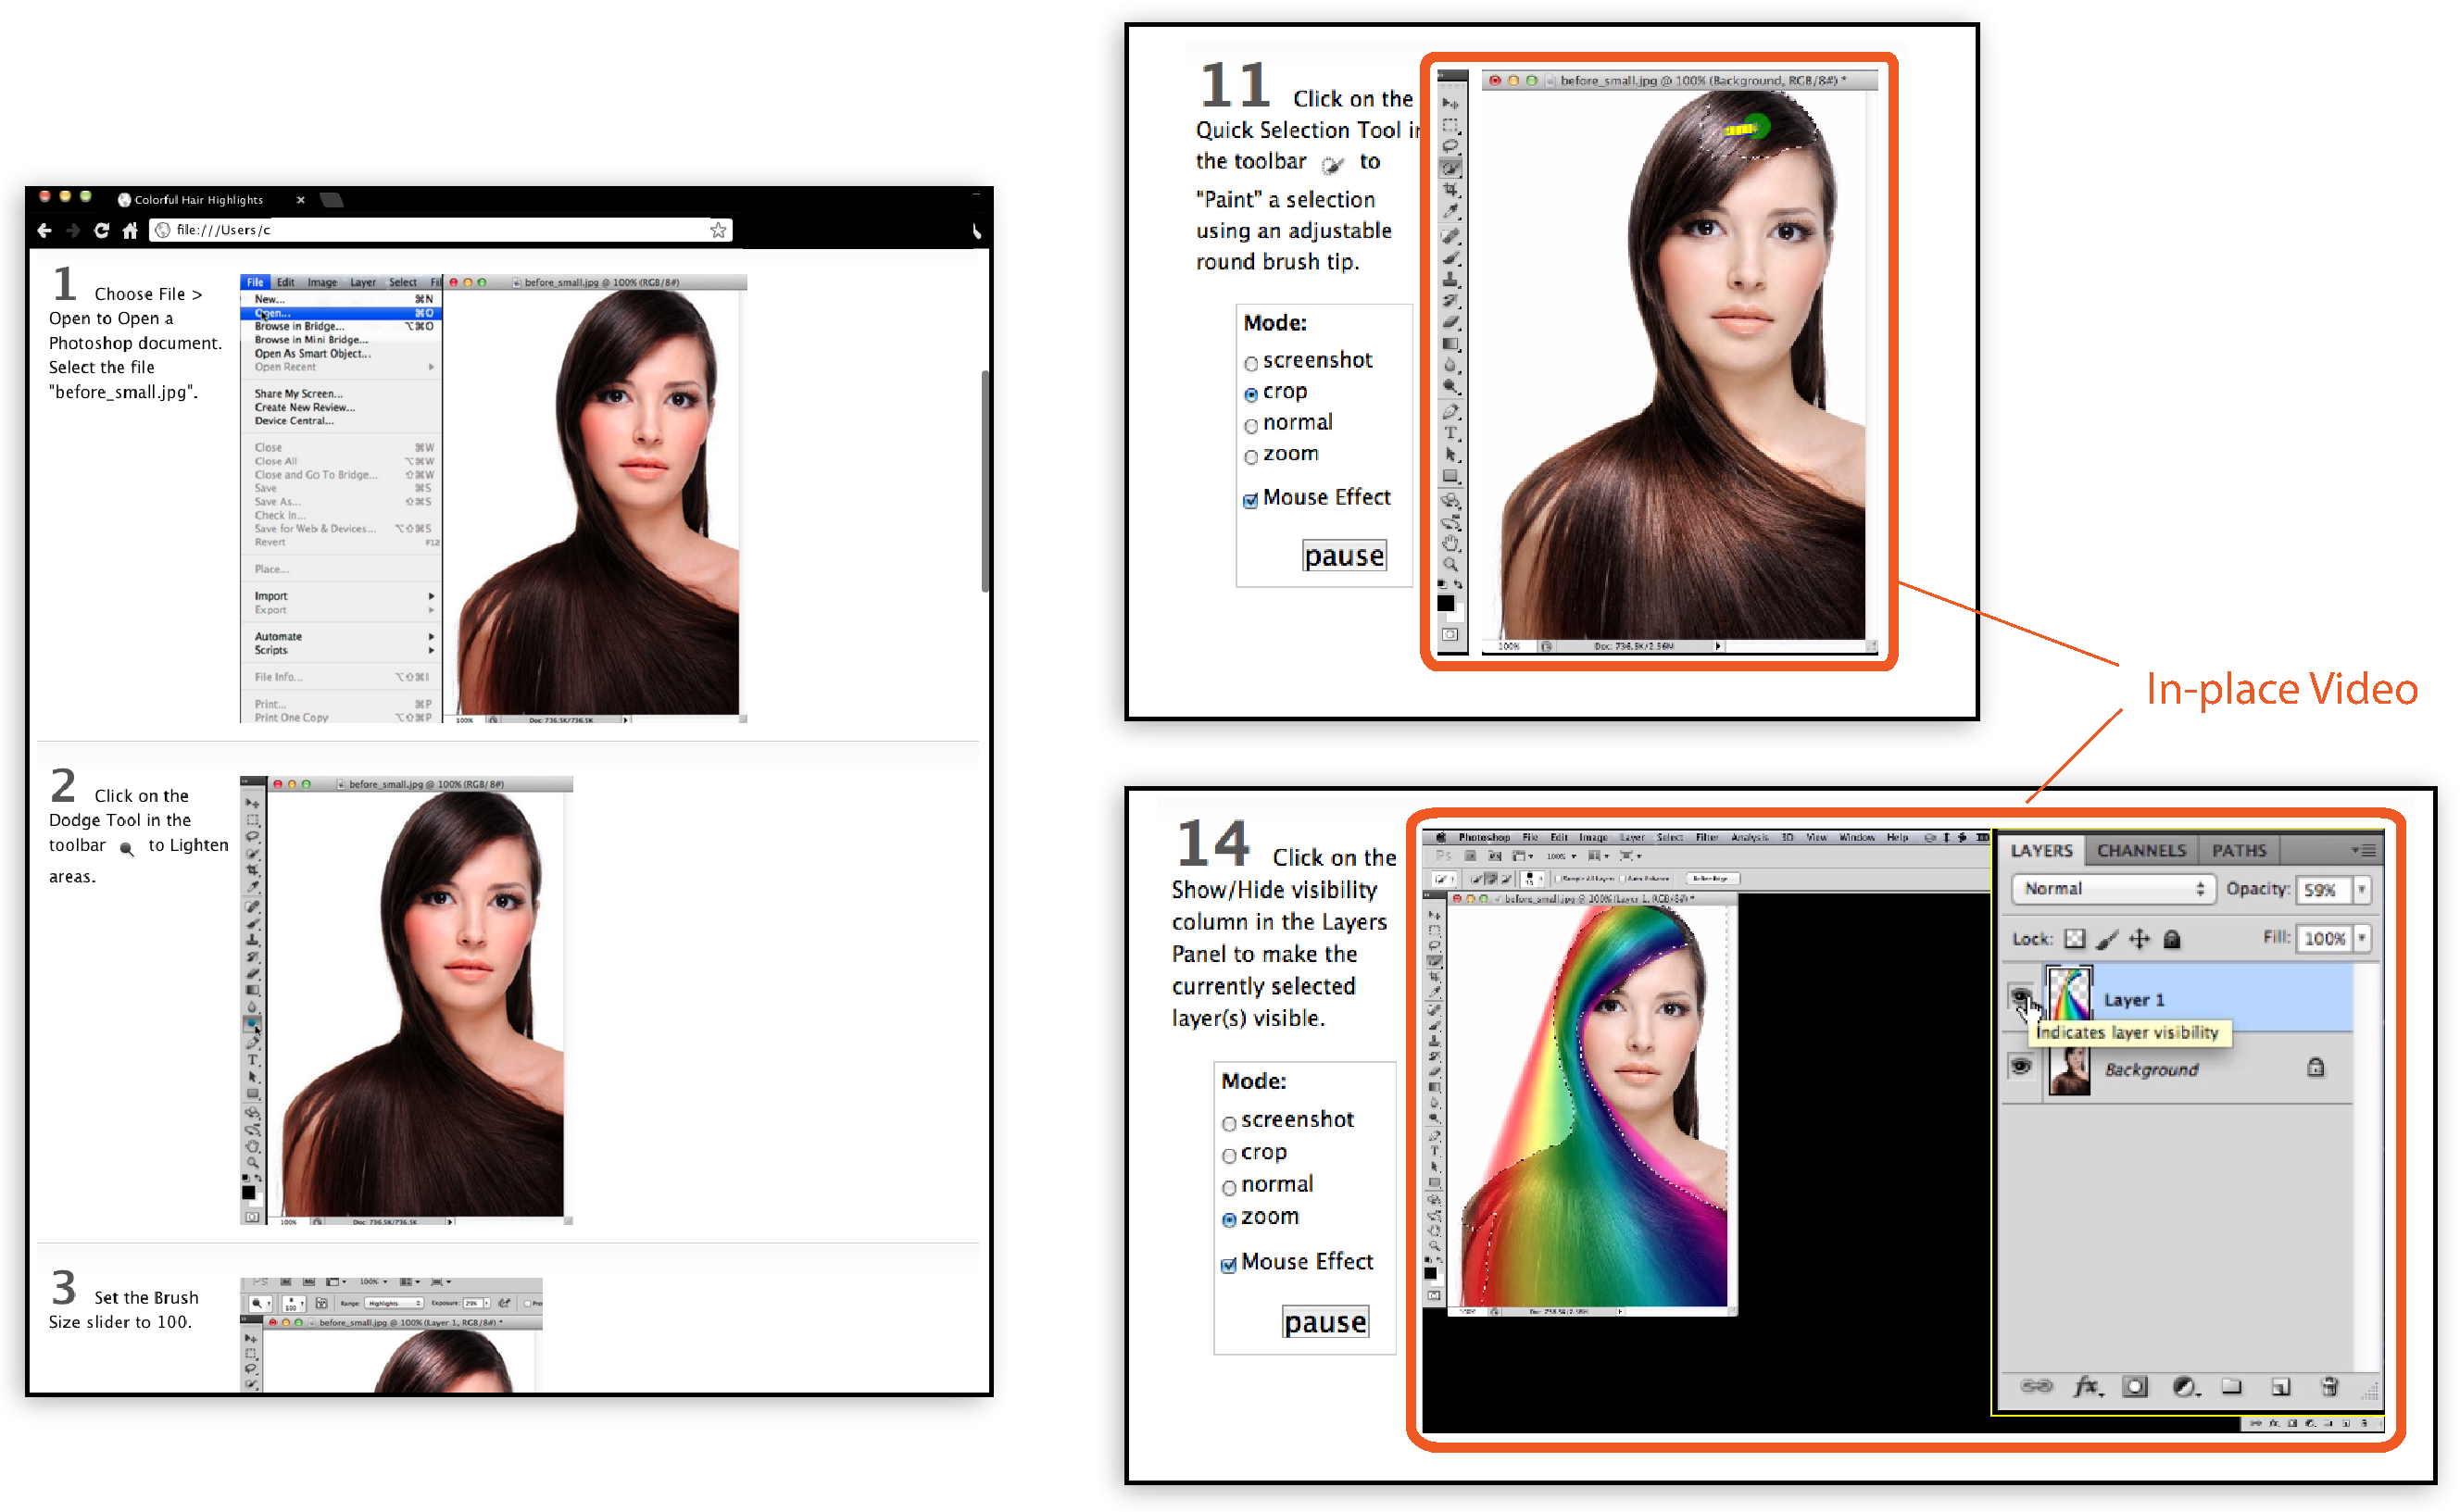
\includegraphics[width=0.8\textwidth]{\intro/fig/mixt_intro}
  \caption{MixT generates step-by-step tutorials (left) that contain static and video information from task demonstrations. Videos are automatically edited and offer different views (right) to highlight the most relevant screen areas for a step. Visualizing mouse movement helps learners understand a complex action.}
  \label{fig:mixt_intro}
\end{figure*}

\subsection{New Tutorial Formats}

Both static and video tutorials have strengths, but neither format alone is well suited for all learning needs that learners may have.
%
To combine the benefits, we design a new instructional presentation called \emph{MixT} (mixed-media tutorials) that improves learners' success in following instructions (see Figure~\ref{fig:mixt_intro}).
%
MixT presents step-by-step static instructions and includes in-place video clips for each operation.
%
With MixT, learners can quickly scan forward and backward on a web page to obtain an overview of a task. Embedded videos help them understand continuous, complex manipulation, such as brushing on a canvas and adjusting control points.
%
MixT's playback UI allows learners to interactively control \emph{when} to see images or videos, and \emph{how} to render videos.
%
Video editing techniques are applied to emphasize instructions, including cropping salient screen regions and highlighting interaction.
%
In our within-subject experiment, MixT successfully reduced numbers of errors and attempts made by learners when following image manipulation tasks.
% To demonstrate , MixT captures screencast video and operation events of a software demonstration.

% ----- DemoWiz ----- %
MixT offers a novel way of navigating instructional content with a combination of static step-by-step and embedded video presentations. If an author wants to narrate over a video recording to illustrate a demo, it can be challenging to pace oneself at the suitable timing without expecting \emph{when} and \emph{what} action is taking while a video is playing.
%
We design \emph{DemoWiz}, a system that augments a screencast video with visualizations (Figure~\ref{fig:demowiz_intro}). By logging the input events of a software demonstration, DemoWiz overlays glyphs to visually guide viewers to the next action along with the time remaining before the action occurs. This enables viewers to anticipate the video content rather than react to it.
%
Our study showed that fewer anticipation errors and narration delays were made with DemoWiz.

\begin{figure*}[t]
\centering
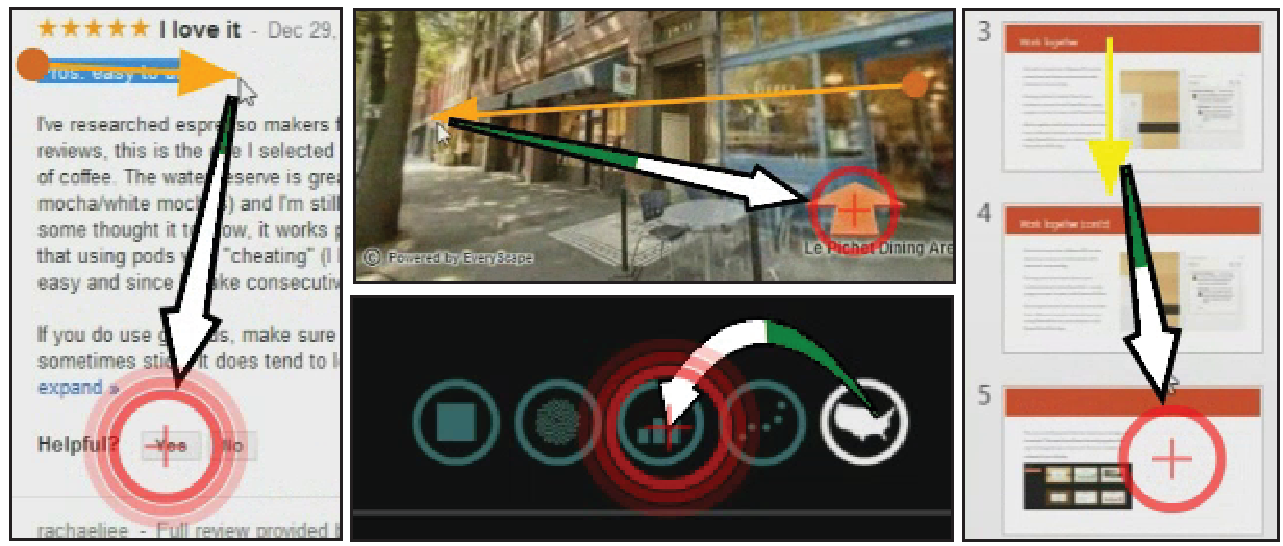
\includegraphics[width=0.7\columnwidth]{\intro/fig/DemoWiz}
\caption{DemoWiz visualizes input events in a screencast video to help viewers anticipate the upcoming event for following a software demonstration.}
\label{fig:demowiz_intro}
\end{figure*}

\subsection{Tutorial Generation from Software Demonstration}

While new tutorial formats are shown to be useful, manually creating instructions can be extremely time- and effort-consuming. In response, we design computational methods to automate the creation process from an author demonstration. MixT and DemoWiz capture screencast video and input device events from a demonstration of a task in a software application. MixT also records application commands for video analysis. Computer vision and visualization techniques are integrated to segment a video into steps, extract salient information, and add visual highlights.
%
In addition, DemoWiz supports an editing phase where authors can adjust the timing of events in a video. Playback speed of recorded actions can be modified or skipped via an editing UI. Our studies showed that our algorithms for step segmentation, event detection, and visualization were effective (\textless8\% error rate in MixT and 0\% in DemoWiz).

\subsection{Interactive Tutorial Authoring from Physical Demonstration}

% ----- DemoCut ----- %

Moving beyond software applications, support for authoring instructions of tasks that take place in the physical world is lacking. Activity recognition remains an open research question, and making authoring decisions during a demonstration can be difficult.
%
To address this problem, we first look into Do it yourself (DIY) project tutorials, which help people learn knowledge and skills to complete a task independently.
%
We developed \emph{DemoCut}, a semi-automatic video editing system that improves the quality of amateur instructional videos for physical tasks (Figure~\ref{fig:democut_intro}). DemoCut asks authors to describe key ``moments'' in a recorded demonstration video using a set of markers. Based on the annotations, our system analyzes the audio and visual activities to automatically organize the video into meaningful segments. Editing decisions are applied to support both \emph{temporal effects} that increase playback speed or skip segments, as well as \emph{visual effects}, such as zooming, subtitles, and visual highlights. A playback interface allows authors to quickly review and edit the automatically generated effects.
%
Our studies showed that video tutorials created by DemoCut in five DIY domains were concise in terms of video length and descriptive instructions with low effect error rates.

\begin{figure*}[t]
  \centering
  \includegraphics[width=\textwidth]{\intro/fig/DemoCut}
  \caption{DemoCut asks authors to mark key moments in a recorded video of demonstration using a set of marker types. Based on marker information, the system uses audio and video analysis to automatically organize the video into meaningful segments and apply appropriate video editing effects, which can be modified via a playback UI.}
  \label{fig:democut_intro}
\end{figure*}

% ----- Kinectograph ----- %
Through the process of designing DemoCut for automatic DIY video editing, we observed that for tasks that require larger space and more movements, instructors often have to adjust the position and viewing angle of a camcorder. Some authors choose to set up multiple cameras and later select the best shot from video streams, while some invite another person who controls the camcorder during a demonstration.
%
To enable authors to record their demonstration without acquiring additional cameras or cameraman, we design \emph{Kinectograph}, a video recording device with a single camera that automatically tracks and follows specific body parts, e.g., hands, of an instructor in a video (see Figure~\ref{fig:kinectograph_intro}). It utilizes a Kinect depth sensor to track skeletal data and adjusts the camera angle via a 2D pan-tilt gimbal mount. Authors can freely move around in space to demonstrate a task and monitor real-time video preview through a tablet application.

\begin{figure}[!t]
  \centering
  \includegraphics[width=0.65\columnwidth]{\intro/fig/Kinectograph}
  \caption{Composed of a Kinect camera to track author movement and a motorized dock to pan and tilt the camera, Kinectograph allows the author (or their hand) remains centered in the recorded video in real-time.}
\label{fig:kinectograph_intro}
\end{figure}

% ----- DemoDraw ----- %

The successful experiences supporting motion-based recordings motivated me to apply our demonstration-based approach to a domain that is entirely driven by movements. In sports, dance performance, and body gesture interfaces, movement instructions are often conveyed with drawings of the human body annotated with arrows or stroboscopic effects~\cite{cutting_representing_2002}. However, current practices require authors to manually sketch or trace subjects from photographs, which is time-consuming and difficult to make changes once created.
%
We design \emph{DemoDraw}, a system that generates concise illustrations from author demonstration (see Figure~\ref{fig:demodraw_intro}). With DemoDraw, an author records one or more motions by physically demonstrating in front of a Kinect sensor. In a multi-modal Demonstration Interface, DemoDraw segments speech and 3D joint motion into a sequence of motion segments, each characterized by a key pose and salient joint trajectories. Based on this sequence, a series of illustrations is automatically generated using a stylistically rendered 3D avatar annotated with arrows to convey movements. Once a suitable sequence of steps has been created, a Refinement Interface enables fine control of visualization parameters.
%
In a three-part evaluation, our results show 4 to 7-step illustrations can be efficiently created in 5 or 10 minutes on average.

\begin{figure}[t]
  \centering
  \includegraphics[width=\columnwidth]{\intro/fig/DemoDraw}
  \caption{DemoDraw's multi-modal approach enables authors to capture motion, verify results, and re-perform portions if needed to generate step-by-step motion illustrations.}
  \label{fig:demodraw_intro}
\end{figure}

% ---------------------------------------------------------------

\section{Thesis Contributions}

Overall, our video-based approaches consider key events or moments that are important to a learner. This information can be derived from software event logs or human annotation of physical tasks when automatic recognition remains challenging. Based on the metadata and video streams, we propose automatic methods to generate concise instructions for two task domains, software applications and physical tasks (see Figure~\ref{fig:space}). Our approaches support authors from recording demonstrations to editing and reviewing system-generated instructions. Interactive controls are available in different stages via desktop or multi-modal interfaces.
%
We demonstrate a series of systems that consider production stages of tutorial creation and learning. We present the rationale and technical challenges of these interactive system designs. Each system is evaluated both quantitatively and qualitatively to study the usability in authoring and learning.

% \clearpage
The contributions of this dissertation include:

\begin{itemize}
\item New instructional formats that consider the learning needs from several domains, including software applications and physical activities.
\item Multi-modal interaction techniques for novice or amateur authors to create effective instructions by demonstration.
\item Automatic or semi-automatic approaches using video and audio analysis that includes authors in the loop to produce high-quality instructions.
\end{itemize}

\begin{figure}[t!]
  \centering
  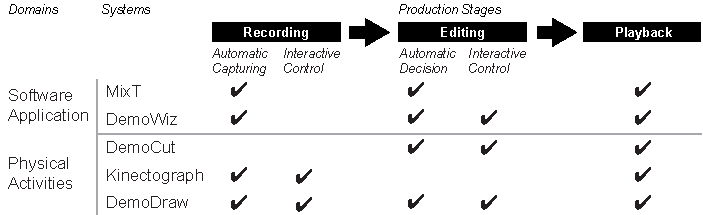
\includegraphics[width=0.9\columnwidth]{\intro/fig/space}
  \caption{A design space of the creation and consumption process for tutorials. It involves three phases of recording, editing, and playback in either software domain or a physical world. This dissertation proposes a series of systems that focus on various aspects in this design space.}
  \label{fig:space}
\end{figure}

% ---------------------------------------------------------------

\section{Overview}

The rest of this dissertation is structured as follows:
%
In Chapter \ref{chapter_background}, we define terminology used in instruction creation and consumption process based on literature. We review studies on why people rely on tutorials in general, how the formats of instructions matter, and the current practices of authoring instructions.
%
In Chapter \ref{chapter_related_work}, we review the literature on research and technologies used in supporting activities of authoring and consuming instructions.

We presented two systems that generate interactive tutorials for software applications.
% MixT
In Chapter \ref{chapter_mixt}, we present our study on how a new tutorial format supports learners in following step-by-step instructions with mixed media, including static text, images, and video clips. We introduce our creation tool called MixT, which automatically generates such new tutorial format from a software demonstration.
% DemoWiz
Chapter \ref{chapter_demowiz} introduces DemoWiz, a system that assists viewers in capturing the timing of input events in a screencast demo video. DemoWiz supports recording, editing, and reviewing stages in a production process with an authoring and playback UI.

Then, we introduced three systems designed for real-world tasks that involve physical demonstrations.
% DemoCut
In Chapter \ref{chapter_democut}, we present a semi-automatic tool for DIY video editing. Our system, called DemoCut, provides two authoring interfaces, annotation and editing, that enable authors to mark a demo video and review and modify the automatically edited results. The design is based on an fundamental understanding of DIY activities.
% Kinectograph
In Chapter \ref{chapter_kinectograph}, we focus on a recording device that automatically follows a demonstrator for filming instructional videos. The Kinectograph system tracks an author's position and body parts and provides an authoring interface for real-time camera control.
% DemoDraw
Finally, in Chapter \ref{chapter_demodraw}, we introduce a multi-modal approach for authors to generate motion illustrations by physically demonstrating the movements. DemoDraw is a system that segments speech and 3D joint motion into a sequence of motion segments and renders effective illustrations. Two authoring interfaces enable authors to navigate, re-perform, and edit visualization parameters.

% Conclusion
Throughout this dissertation, we discuss how our video-based approaches increase the quality of amateur-produced video instructions. Chapter \ref{chapter_conclusion} concludes our work on tutorial creation and consumption in both software and physical instructions. New directions for future research on interactive tutorials are proposed.

% ---------------------------------------------------------------

\section {Prior Publications}

This dissertation is based on papers published in previous ACM conference proceedings: the MixT system was published at UIST 2012~\cite{Chi:2012:MAG:2380116.2380130}, DemoWiz at CHI 2014~\cite{Chi:2014:DRS:2556288.2557254}, DemoCut at UIST 2013~\cite{Chi:2013:DGC:2501988.2502052}, and Kinectograph at CHI 2013~\cite{Cheng:2013:BCC:2468356.2468568}; DemoDraw will be published at UIST 2016~\cite{Chi:2016:DemoDraw}.

While I am primary author on all publications and led the described projects, this research could not have been completed without my advisor Bj\"orn Hartmann and my collaborators that I have been fortunately to work with. Specifically, Dr. Mira Dontcheva and Dr. Wilmot Li at Adobe Research provided valuable guidance on three projects (MixT, DemoCut, and DemoDraw); Dr. Steven M. Drucker and Dr. Bongshin Lee at Microsoft Research guided the DemoWiz project with their expertise on visualization; Professor Daniel Vogel at University of Waterloo greatly contributed to the DemoDraw project. A group of MS and undergrad students at UC Berkeley and Adobe contributed to implementation, design, and user study in the projects, including Sally Ahn and Amanda Ren in MixT, Joyce Liu and Jason Linder in DemoCut, and Derrick Cheng and Taeil Kwak in Kinectograph.

% We are all natural performers. Humans are proficient at demonstrating how to perform a task in action. However, articulating knowledge into a written or structured form can be extremely difficult. From dancing, repairing a machine, to operating software applications, it remains a challenge how everyday activities can be efficiently captured for a remote learner to understand.
